\documentclass{article}
\usepackage[utf8]{inputenc}
\usepackage{graphicx, amsmath, amssymb}
\usepackage{hyperref}
\graphicspath{ {./images/} }
\usepackage[dvipsnames]{xcolor}

\title{Self-Attention and Transformers}
\author{sumit singh}
\date{\today}

\begin{document}

\maketitle
\begin{abstract}
\noindent
This is a test. That is an abstract.  T This is a test. That is an abstract. 

\end{abstract}

\hspace{0.5in}
\keywords{Postional Encoding, Rotary Positional Embeddings, Positional Embeddings, Context Vectors}
%*********************************************************************************************
\section{Motivation for Transformers}
\begin{itemize}
    \item Sequential computation prevents parallelization
    \item Despite GRUs and LSTMs, RNN still need attention mechanism to deal with long-range dependencies - path length for co-dependent computation between states grows with sequence length
    \item But if attention gives us access to any state, maybe we don't need the RNN?!
\end{itemize}

%*********************************************************************************************    
\section{Transformers}
%*********************************************************************************************   
\begin{minipage}{0.5\textwidth}
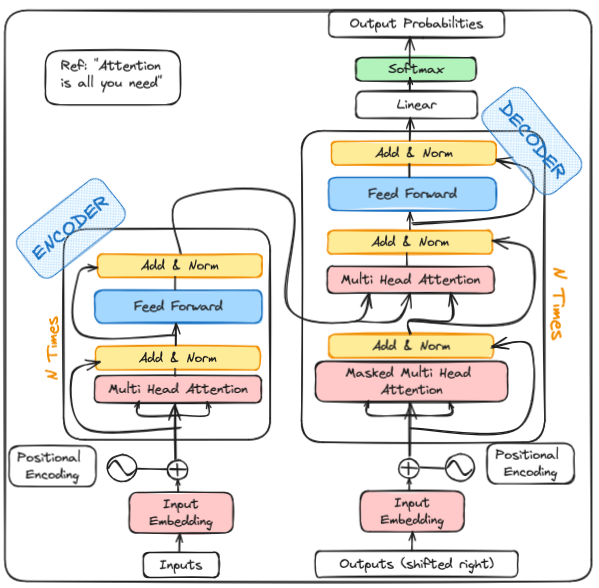
\includegraphics[width=6cm, height=8cm]{Transformer/Images/Transformers1.png}
\end{minipage}
\begin{minipage}{0.5\textwidth}
\begin{itemize}
    \item The work "Attention is All you Need" (Vaswani et al, NeurIPS 2017) first made it possible to do Seq2Seq modelling without RNNs)
    \item Proposed transformer model, entirely built on self-attention mechanism without using sequence-aligned recurrent architectures
    \item Key components:
    \begin{itemize}
        \item Self-Attention
        \item Multi-Head Attention
        \item Positional Encoding
        \item Encoder-Decoder Architecture
    \end{itemize}
\end{itemize}
\end{minipage}
%************************************************************************************
\subsubsection{Transformers in a Nutshell}
\begin{minipage}{0.5\textwidth}
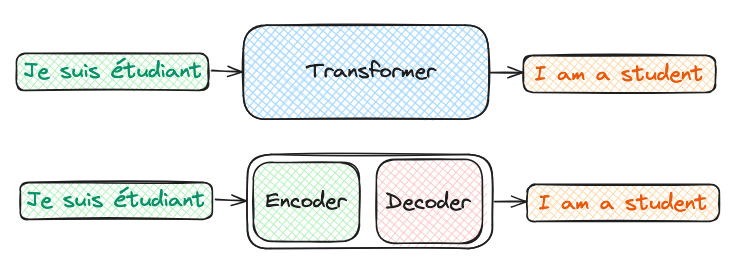
\includegraphics[width=6cm, height=3cm]{Transformer/Images/Transformers2.png}
\end{minipage}
\begin{minipage}{0.5\textwidth}
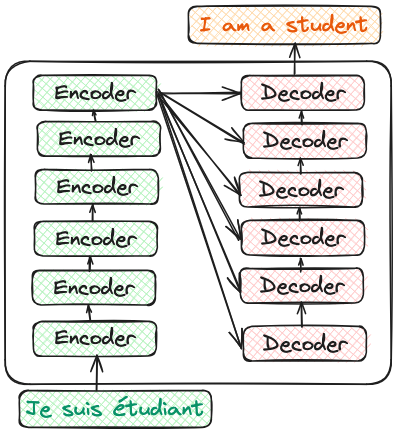
\includegraphics[width=6cm, height=5cm]{Transformer/Images/Transformers3.png}
\end{minipage}
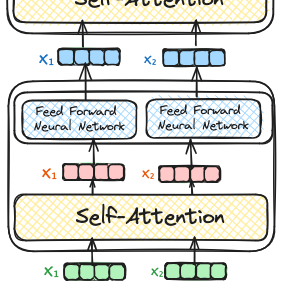
\includegraphics[width=6cm, height=6cm]{Transformer/Images/Transformers4.png}
%************************************************************************************
%************************************************************************************
\section{Self-Attention}
%************************************************************************************
\begin{itemize}
    \item Consider two input sentences we want to translate:
    \begin{itemize}
        \item The \textcolor{red}{animal} didn't cross the street because it was too \textcolor{red}{tired}
        \item The animal did not cross the  \textcolor{red}{street} because it was too \textcolor{red}{wide}
    \end{itemize}
    \item "it" refers to "animal" in the first case, but to "street" in the second case
    \item This is hard for traditional \textit{Seq2Seq} models to model.
    \item As the model processes each word, self-attention allows it to look at other positions in the input sequence to help get a better encoding. 
    \item Recall RNNs: we now no longer need to maintain a hidden state to incorporate representation of previous words/vectors!
\end{itemize}
%************************************************************************************
\begin{minipage}{0.5\textwidth}
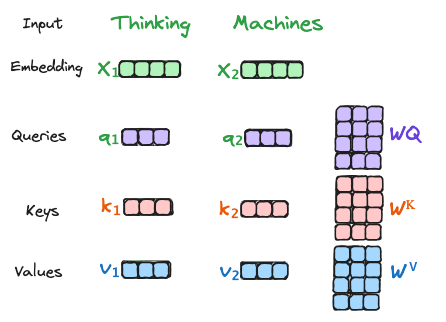
\includegraphics[width=6cm, height=6cm]{Transformer/Images/SelfAttention1.png}
\end{minipage}
\begin{minipage}{0.5\textwidth}
\begin{itemize}
    \item \textbf{STEP 1}: Create three vectors from encoder's input vector ($x_i$):
    \begin{itemize}
        \item Query vector ($q_i$)
        \item Key vector ($k_i$)
        \item Value vector ($v_i$)
    \end{itemize}
    \item These are created by multiplying input with weight matrices $W^Q, W^K, W^V$, learned during training.
    \item In the paper $q,k,v \in \mathbb{R}^{64} $ and $x \in \mathbb{R}^{512}$
    \item Do $q,k,v$ always have to be smaller than $x$? No, this was done perhaps to make computation of multi-headed attention constant
    \item What are the dimensions of $W^Q, W^K, W^V$?
\end{itemize}
\end{minipage}
\\
%************************************************************************************
\begin{minipage}{0.5\textwidth}

\begin{itemize}
    \item \textbf{STEP 2}: Calculate self-attention scores - Score all words of input sequence against themselves. How?
    \item By taking dot product of \textcolor{blue}{query vector} with \textcolor{blue}{key vector} of respective words
    \item E.g. for input "Thinking", first score would be $q_1 \cdot k_1 $
    \item  (with itself); second score would be dot product of $q_1 \cdot k_2$ (with "Machines"), and so on.
    \item Scores then divided by $\sqrt{length(k)}$
    \item This is \textcolor{blue}{Scaled Dot-Product Attention},. This design choice leads to more stable gradients.
\end{itemize}
\end{minipage}
\begin{minipage}{0.5\textwidth}
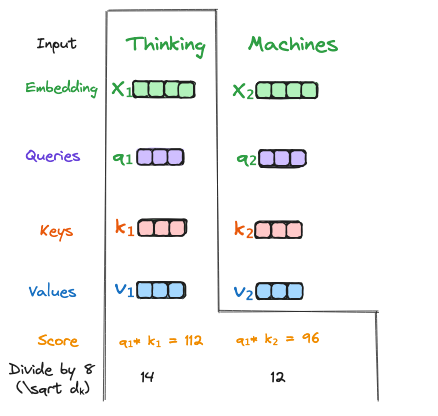
\includegraphics[width=6cm, height=6cm]{Transformer/Images/SelfAttention2.png}
\end{minipage}
%************************************************************************************
\begin{minipage}{0.5\textwidth}
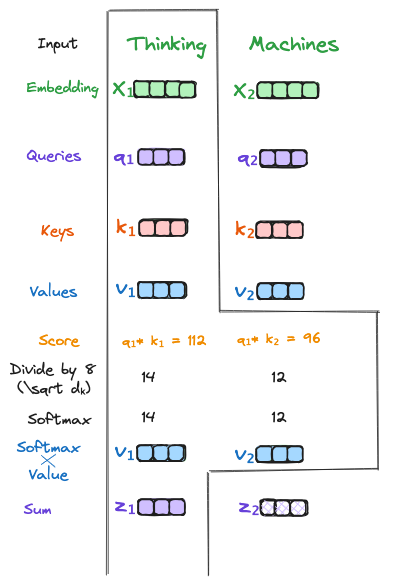
\includegraphics[width=6cm, height=8cm]{Transformer/Images/SelfAttention3.png}
\end{minipage}
\begin{minipage}{0.5\textwidth}
\begin{itemize}
    \item \textbf{STEP 3}: Softmax used to get normalized probability scores; determine how much each word will be expressed at this position
    \item Clearly, word at this position will have highest softmax score, but sometimes it's useful to attend to another word that is relevant
    \item \textbf{STEP 4}: Multiply each \textcolor{blue}{value vector} by softmax score. Why? Keep value of word(s) we want to focus on intact, and drawn out irrelevant words
    \item \textbf{STEP 5}: Sum up weighted value vectors $\rightarrow$  produces output of self-attention layer at this position (for first word)
\end{itemize}
\end{minipage}
%************************************************************************************
\begin{minipage}{0.5\textwidth}
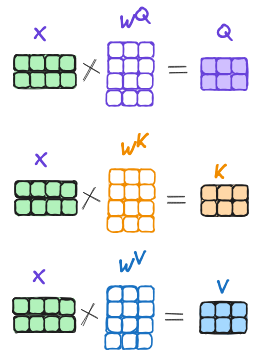
\includegraphics[width=6cm, height=5cm]{Transformer/Images/SelfAttention4.png}
\end{minipage}
\begin{minipage}{0.5\textwidth}
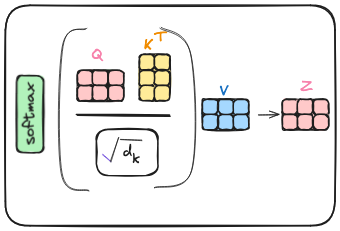
\includegraphics[width=6cm, height=5cm]{Transformer/Images/SelfAttention5.png}
\end{minipage}

%************************************************************************************
%************************************************************************************
\section{Multi-Head Attention}
%************************************************************************************
%************************************************************************************
\begin{minipage}{0.5\textwidth}
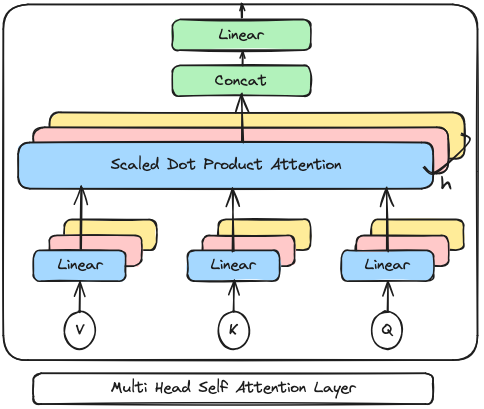
\includegraphics[width=6cm, height=8cm]{Transformer/Images/MultiHeadAttention1.png}
\end{minipage}
\begin{minipage}{0.5\textwidth}
\begin{itemize}
    \item Improves performance of teh attention layer in two ways:
    \begin{itemize}
        \item Expands model's ability to focus on different positions. In example above, $z_1$ contains a bit of every other encoding, but dominated by actual word itself.
        \item Gives attention layer multiple "representation subspaces"; we have not one but multiple sets of Query/Key?value weight matrices; after training, each set is used to project input embeddings into different representation subspaces
    \end{itemize}
\end{itemize}
\end{minipage}
%************************************************************************************
\begin{minipage}{0.5\textwidth}
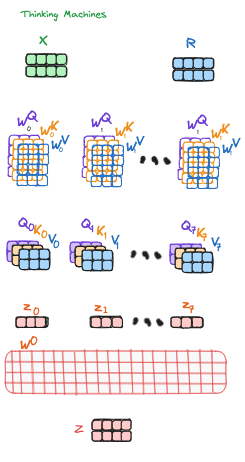
\includegraphics[width=6cm, height=10cm]{Transformer/Images/MultiHeadAttention2.png}
\end{minipage}
\begin{minipage}{0.5\textwidth}
\begin{itemize}
    \item This is our input sequence *
    \item We embed each word * \\
    \item Split into 8 heads. We multiply \textcolor{green}{X} or \textcolor{blue}{R} with weight matrices.
    \item Calculate attention using the resulting \textcolor{pink}{Q}/ \textcolor{orange}{K}/ \textcolor{blue}{V} matrices
    \item Concatenate the resulting \textcolor{pink}{Z} matrices, then multiply with weight matrix \textcolor{pink}{$W^0$} to produce the output of the layer
\end{itemize}
\end{minipage}
*In all encoders other than #0, we don't need embedding. We start directly with the output of the encoder right below this one.
%************************************************************************************
%************************************************************************************
\section{Positional Encoding}
%************************************************************************************
%************************************************************************************
\begin{itemize}
    \item Unlike RNN and CNNN encoders, attention encoder outputs do not depend on order of inputs (Why?)
    \item But order of sequence conveys important information for machine translation tasks and language modeling
    \item The idea: Add positional information of input token in the sequence into input embedding vectors
\end{itemize}
\begin{align*}
    &PE_{pos,2i}   &= sin \frac{pos}{1000^{\frac{2i}{d_{emb}}}} \\
    &PE_{pos,2i+1} &= cos \frac{pos}{1000^{\frac{2i}{d_{emb}}}}
\end{align*}
\begin{itemize}
    \item Final input embeddings are concatenation of learnable embedding and positional encoding
\end{itemize}
%************************************************************************************
%************************************************************************************
\section{References}
%************************************************************************************
\begin{itemize}
    \item \href{https://www.youtube.com/watch?v=phOc25QfNS0&t=55s}{NPTEL Lecture}
    \item \href{https://courses.cs.washington.edu/courses/cse543/22sp/schedule/lecture15_transformer.pdf}{CS Washington}
    \item \href{https://www.youtube.com/watch?v=5V9gZcAd6cE}{Positional encodings in transformers (NLP817 11.5)}
    \item \href{https://www.cs.ubc.ca/~schmidtm/Courses/440-W22/L20.pdf}{CPSC 440}
\end{itemize}
\end{document}